%% CHAP. Intro

\begin{figure}[h]
\centering
  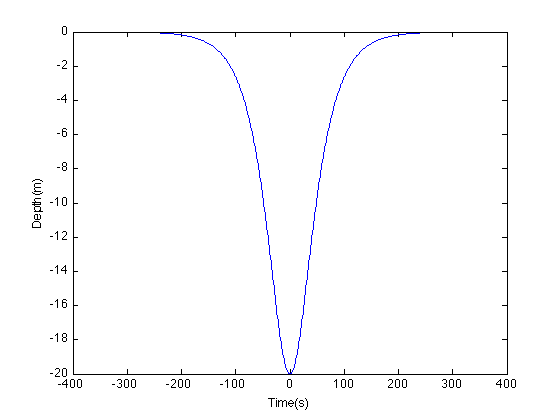
\includegraphics[width=0.8\textwidth]{apel_solution.png}\\
  \caption{Two-layer model of an internal solition.}
  \label{fig:moorings}
\end{figure}



\begin{figure}[h]
\centering
  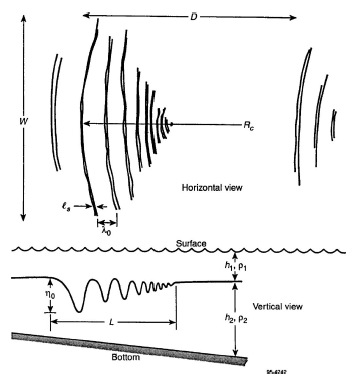
\includegraphics[width=0.8\textwidth]{IW.jpg}\\
  \caption{Internal solitary waves}
  \label{fig:moorings}
\end{figure}


%%CHAP. Ocean


\begin{figure}[h]
\centering
  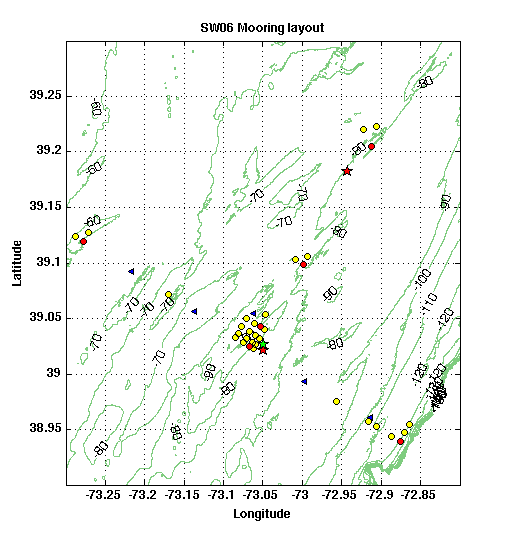
\includegraphics[width=0.8\textwidth]{sw06_mooring.png}\\
  \caption{SW06 mooring locations}
  \label{fig:moorings}
 \end{figure}


\begin{figure}[h]
\centering
  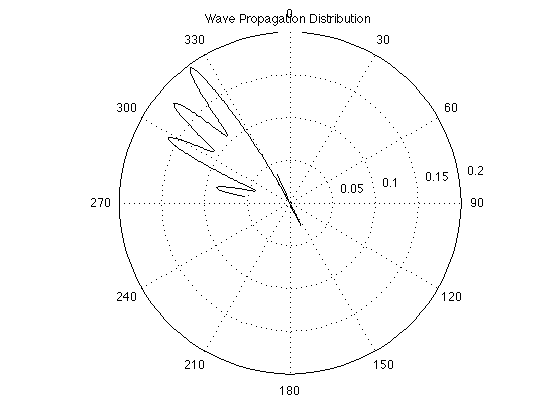
\includegraphics[width=0.8\textwidth]{IW_dir.png}\\
  \caption{Angular distribution of the direction of the internal wave recored during SW06. }
  \label{fig:IW_dir}
\end{figure}


\begin{figure}[h]
\centering
  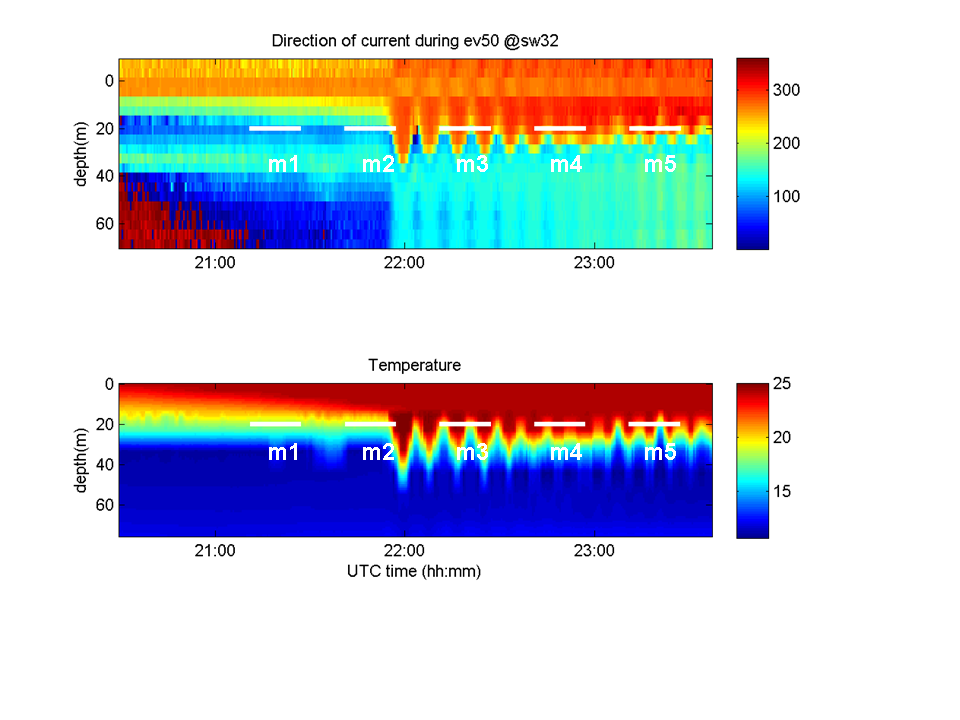
\includegraphics[width=\textwidth]{sw32adcp_temp.png}\\
  \caption{Current data record by ADCP at mooring SW32 during event 50 in SW06 experiment (upper panel) and  temperature data at the same location. }
  \label{fig: sw32adcp_temp}
\end{figure}

%%CHAP. Theory

\begin{figure}[h]
\centering
  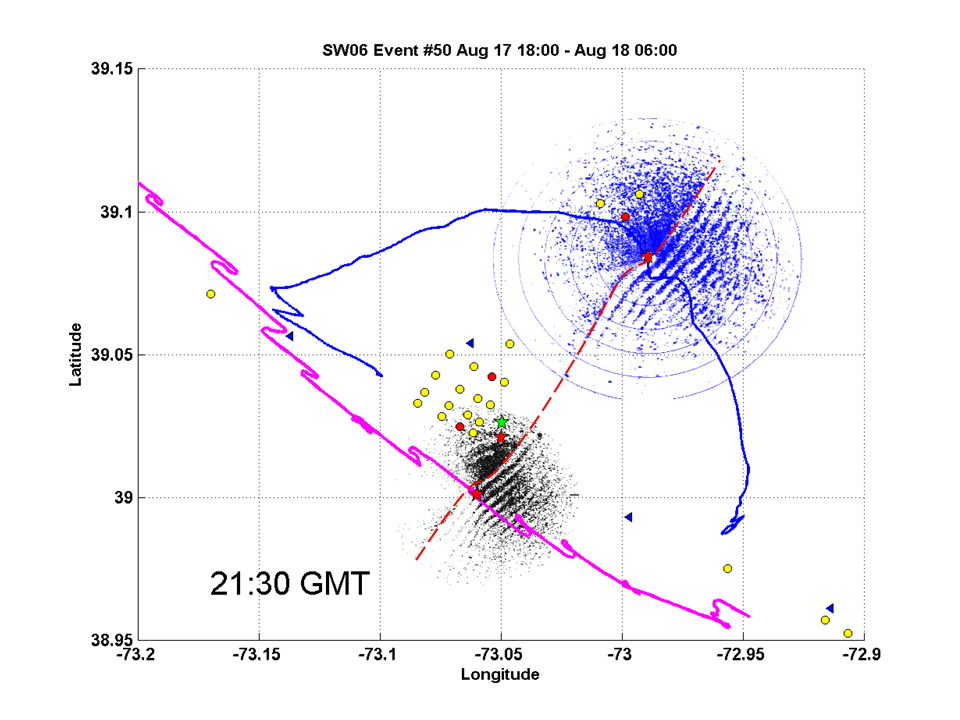
\includegraphics[width=0.8\textwidth]{IW_radar2.png}\\
  \caption{Radar image of internal wave surface signature at 21:30GMT . }
  \label{fig:IW_radar2}
\end{figure}

\begin{figure}[h]
\centering
  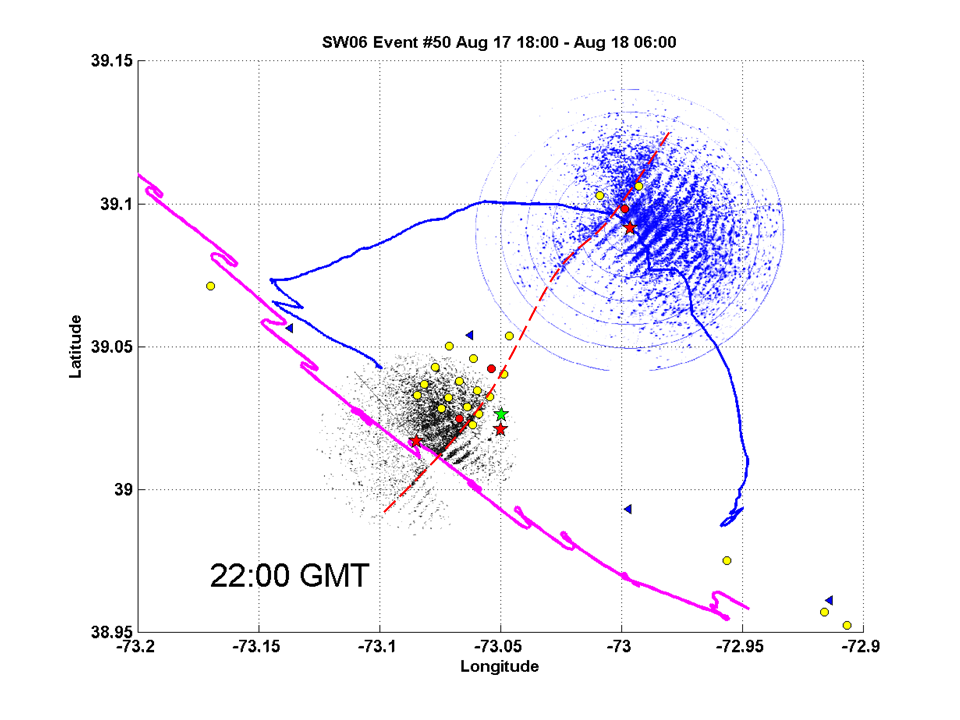
\includegraphics[width=0.8\textwidth]{IW_radar1.png}\\
  \caption{Radar image of internal wave surface signature at 22:00GMT . }
  \label{fig:IW_radar1}
\end{figure}

 \begin{figure}[h]
\centering
  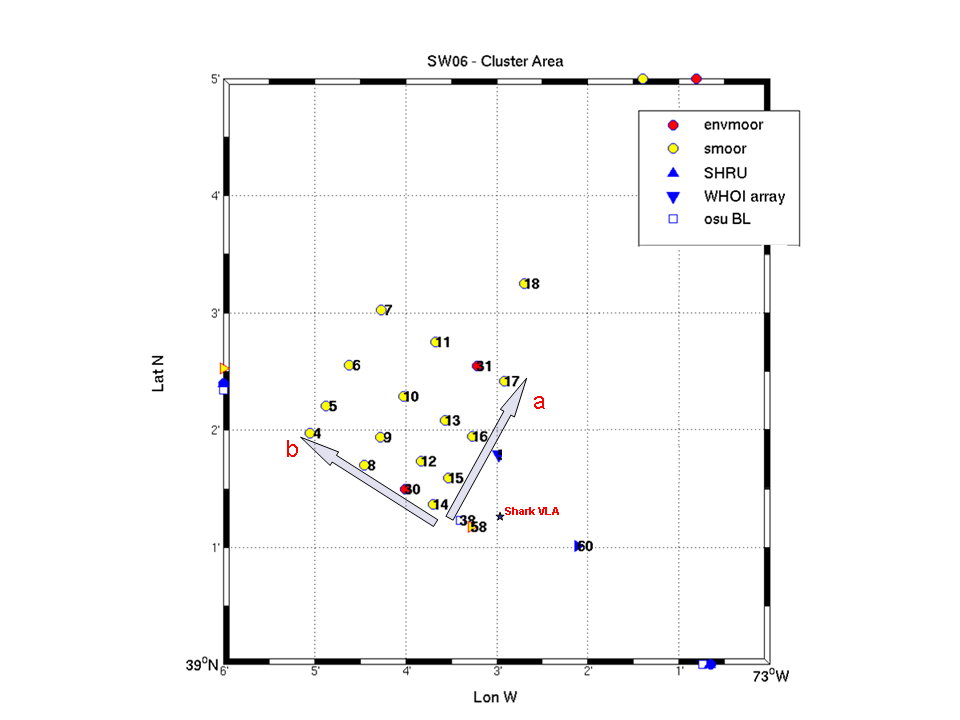
\includegraphics[width=0.8\textwidth]{T_farm2.png}\\
  \caption{Thermistor farm deployed in SW06. Edge (a) \& (b) are parallel and perpendicular to the internal wave fronts, respectively. }
  \label{fig:tfarm}
\end{figure}

 \begin{figure}[h]
\centering
  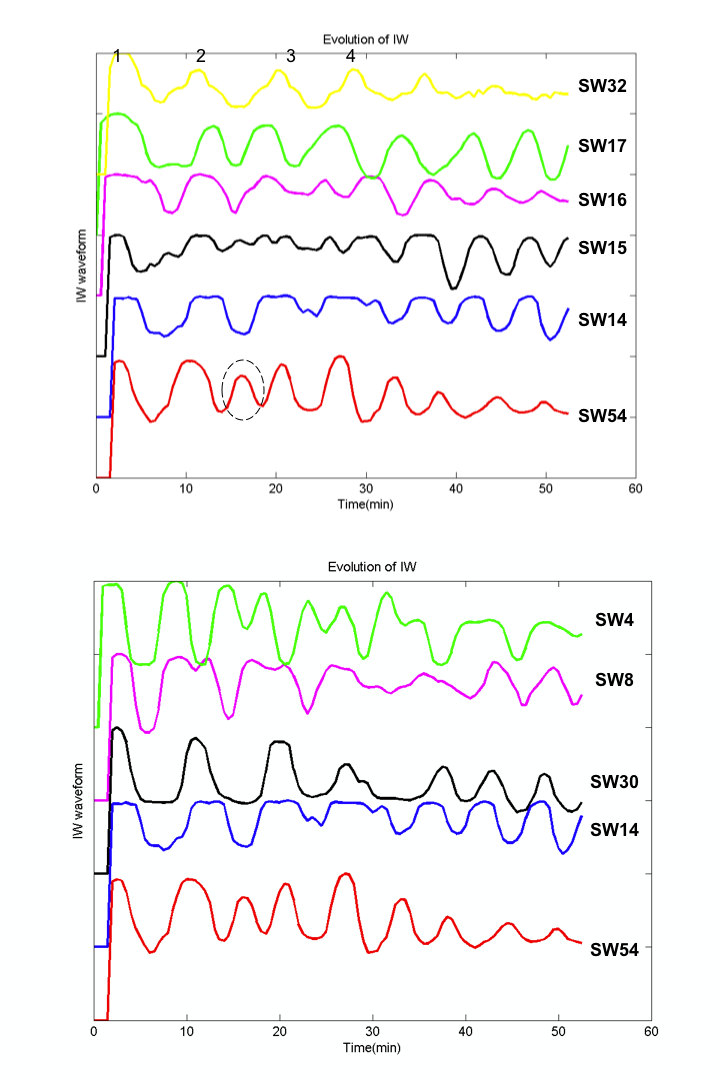
\includegraphics[width=0.8\textwidth]{tfarm_iw.png}\\
  \caption{Temperature data recorded by the thermistor farm during SW06 event 50. }
  \label{fig:tfarm_dir}
\end{figure}

\begin{figure}[h]
\centering
  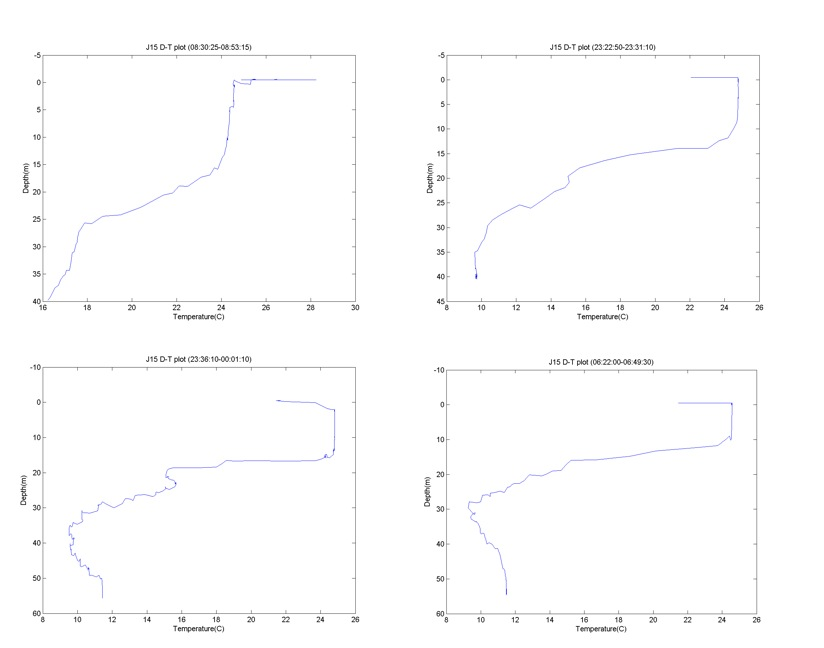
\includegraphics[width=0.8\textwidth]{water_temp4.jpg}\\
  \caption{Temperature profile recorded by TD sensor attached to J15 transducer}
  \label{fig:water_temp4}
\end{figure}

\begin{figure}[h]
\centering
  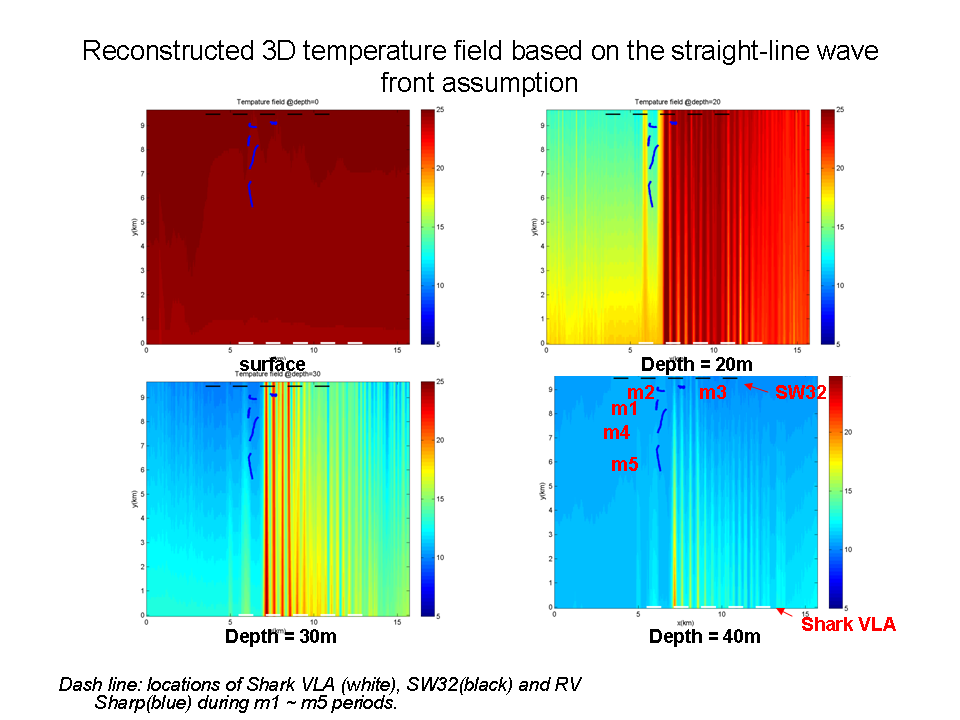
\includegraphics[width=0.8\textwidth]{3D_temp_recon.png}\\
  \caption{Reconstructed temperature field and the movement of source and receiver in the internal wave coordinates}
  \label{fig:water_temp4}
\end{figure}

\begin{figure}[h]
\centering
  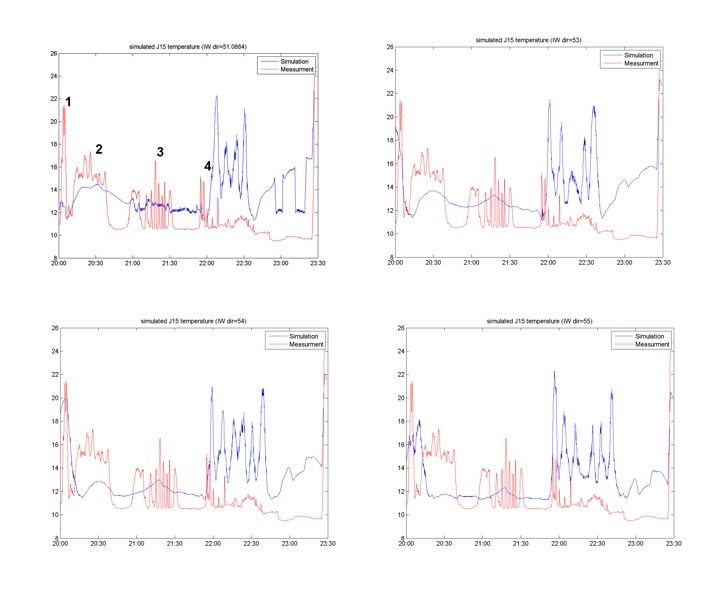
\includegraphics[width=0.8\textwidth]{J15_sim.jpg}\\
  \caption{Simulated J15 recored in reconstructed 3D environment}
  \label{fig:water_temp4}
\end{figure}

\begin{figure}[h]
\centering
  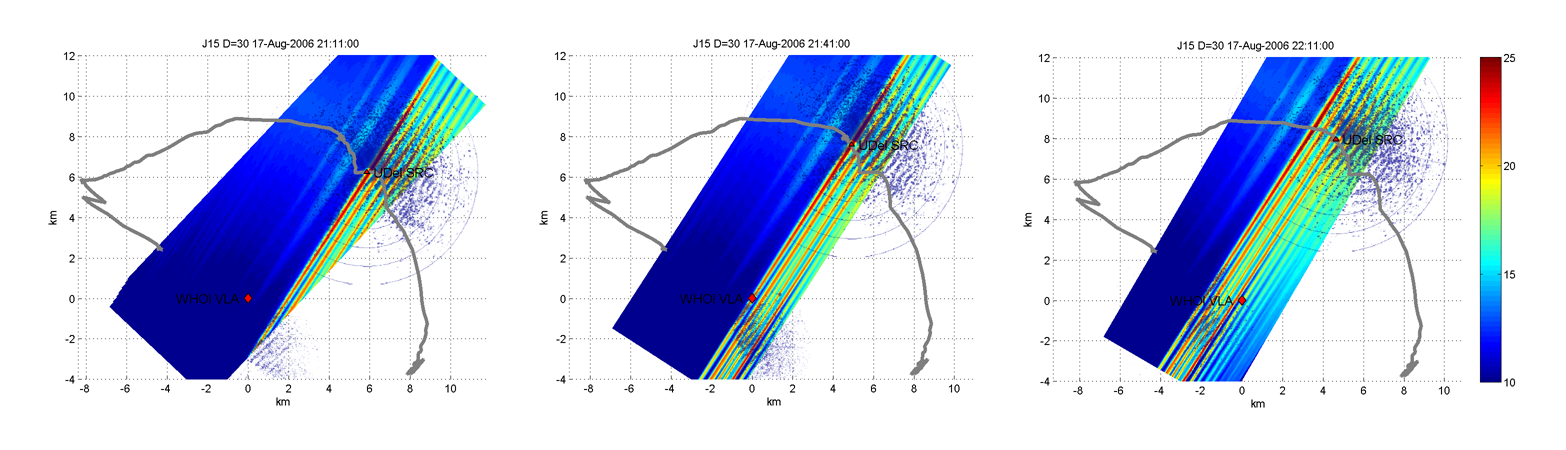
\includegraphics[width=\textwidth]{3D_interp_radar.png}\\
  \caption{Reconstructed temperature field (depth = 30m) with radar image overlay at GMT21:11, 21:41 \& 22:11, Aug 17th.}
  \label{fig: 3D_interp_radar}
\end{figure}

%%CHAP. SW06



\clearpage
%%--F1
\begin{figure}[h]
  \centering
  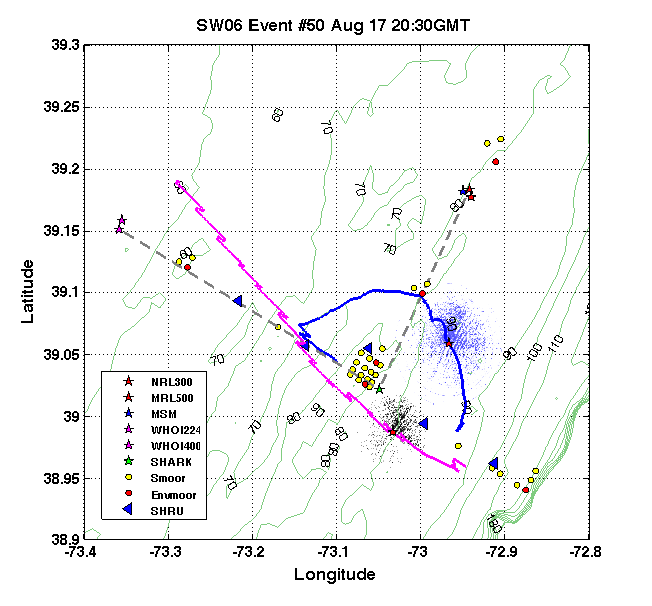
\includegraphics[width=\textwidth]{Aug17_2030_t.png}
  \caption{Surface expression of internal wave package at 21:30GMT, Aug. 17, recorded by R/V Sharp and R/V Oceanus. Blue and red lines indicate their movements, respectively. (Blue: R/V Sharp's, red: R/V Oceanus'}\label{fig:r2130_r}
\end{figure}

\begin{figure}[h]
  \centering
  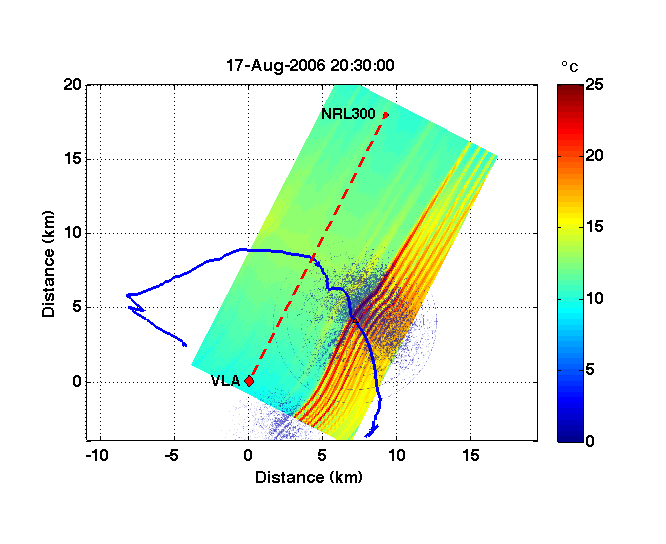
\includegraphics[width=\textwidth]{sw06_Tempr_Depth30m_2006Aug17_203000_radar_curve_thesis1.png}
  \caption{Interpolated internal wave field at 21:30GMT, Aug. 17, water depth = 20m. (Refer to section 3.4 for detailed interpolation method)}\label{fig:r2130_i}
\end{figure}

\begin{figure}[h]
  \centering
  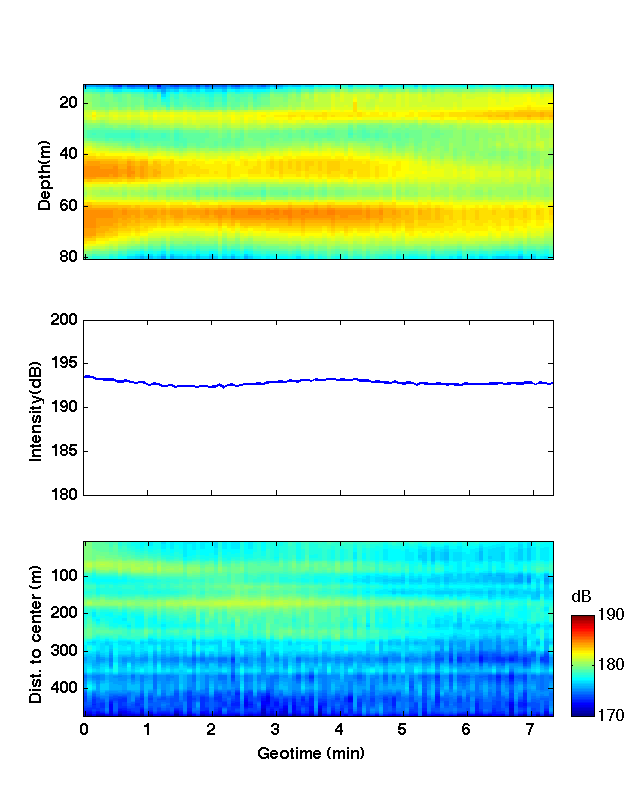
\includegraphics[width=\textwidth]{nrl300_060817T2030_vla_hla_intens_geotime2.png}
  \caption{Received signal on Shark VLA (top), HLA (bottom) and signal intensity (middle) from Aug.17 21:30GMT to 21:37GMT }\label{fig:a2130}
\end{figure}

\begin{figure}[h]
  \centering
  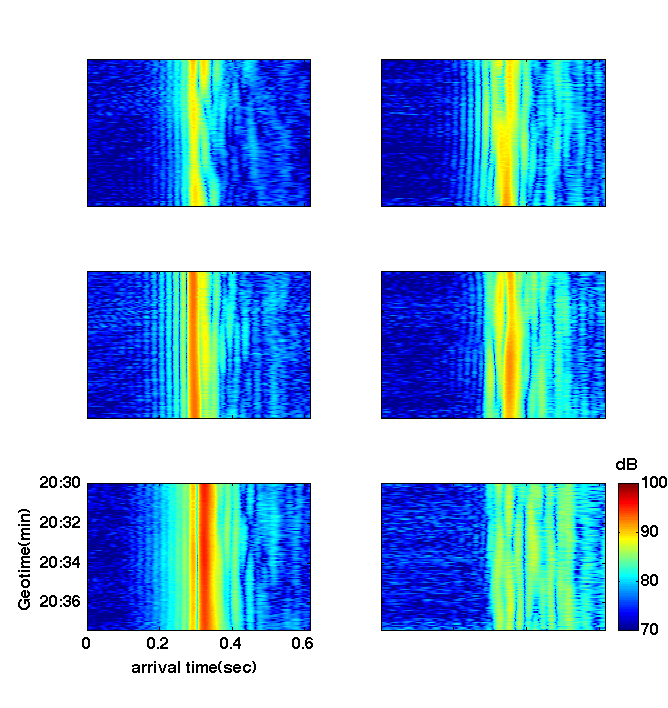
\includegraphics[width=\textwidth]{sw06_broadband_mf_nrl300_F1_6in1_thesis.png}
  \caption{Mode decomposition of received signal on Shark VLA. 
    Left column: mode 1-3, right column: mode 4-6 }\label{fig:m2130}
\end{figure}



%%--F2
\begin{figure}[h]
  \centering
  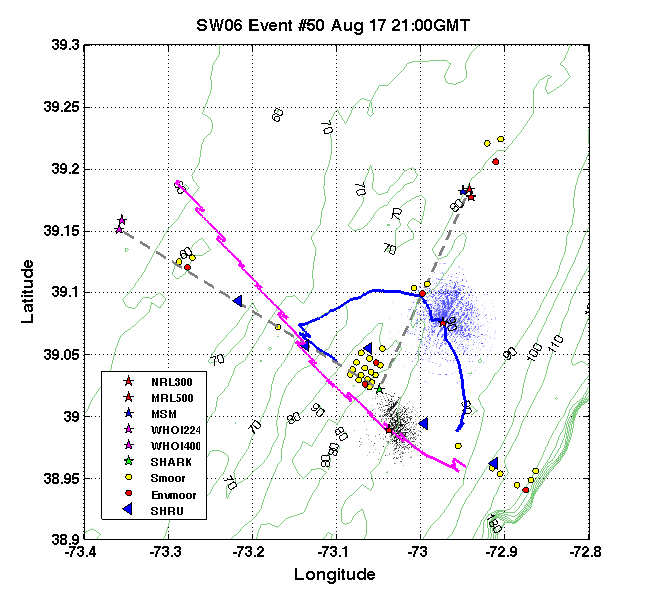
\includegraphics[width=\textwidth]{Aug17_2100_t.png}
  \caption{Surface expression of internal wave package at 21:30GMT, Aug. 17, recorded by R/V Sharp and R/V Oceanus. Blue and red lines indicate their movements, respectively. (Blue: R/V Sharp's, red: R/V Oceanus'}\label{fig:r2130_r}
\end{figure}

\begin{figure}[h]
  \centering
  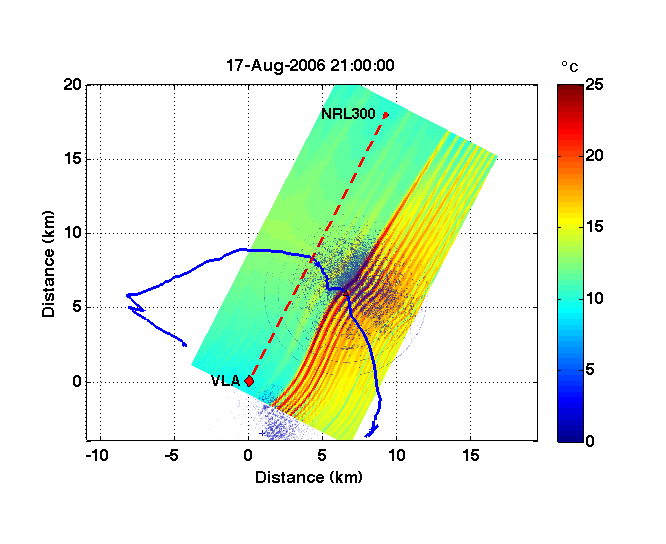
\includegraphics[width=\textwidth]{sw06_Tempr_Depth30m_2006Aug17_210000_radar_curve_thesis1.png}
  \caption{Interpolated internal wave field at 21:30GMT, Aug. 17, water depth = 20m. (Refer to section 3.4 for detailed interpolation method)}\label{fig:r2130_i}
\end{figure}

\begin{figure}[h]
  \centering
  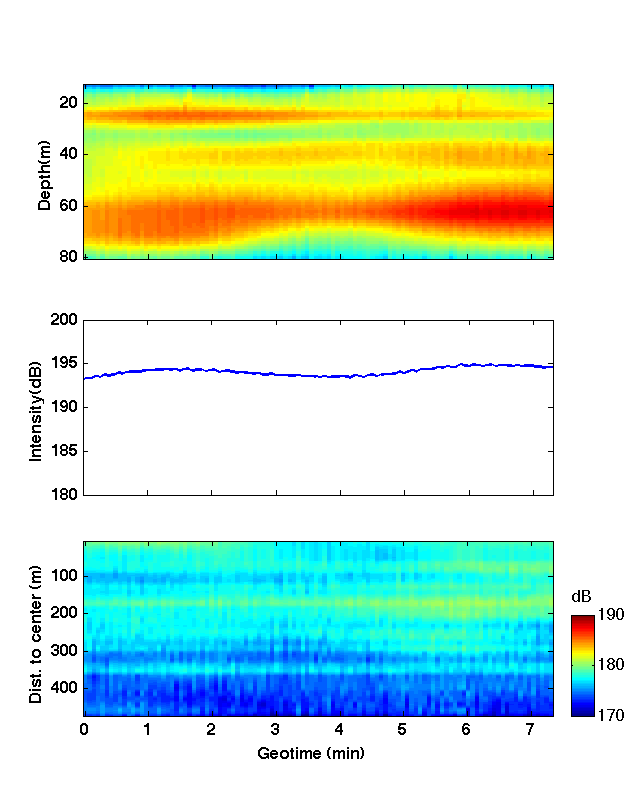
\includegraphics[width=\textwidth]{nrl300_060817T2100_vla_hla_intens_geotime2.png}
  \caption{Received signal on Shark VLA (top), HLA (bottom) and signal intensity (middle) from Aug.17 21:30GMT to 21:37GMT }\label{fig:a2130}
\end{figure}

\begin{figure}[h]
  \centering
  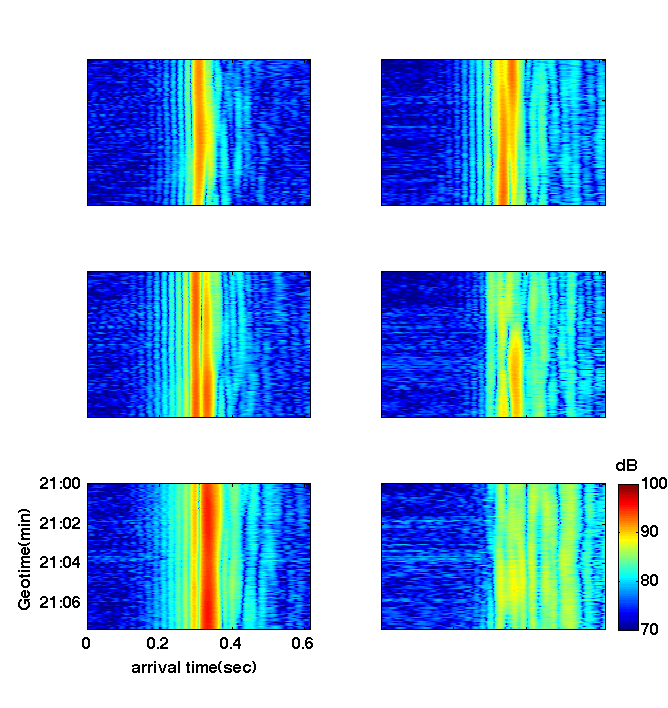
\includegraphics[width=\textwidth]{sw06_broadband_mf_nrl300_F2_6in1_thesis.png}
  \caption{Mode decomposition of received signal on Shark VLA. 
    Left column: mode 1-3, right column: mode 4-6 }\label{fig:m2130}
\end{figure}



%--F3
\begin{figure}[h]
  \centering
  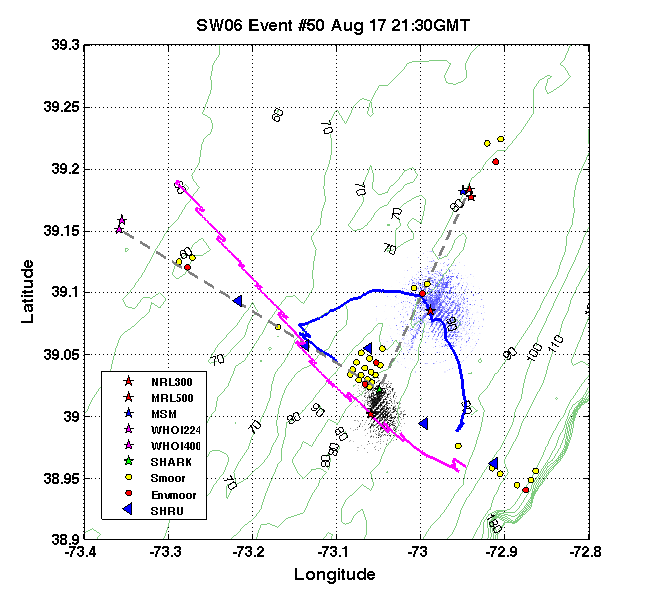
\includegraphics[width=\textwidth]{Aug17_2130_t.png}
  \caption{Surface expression of internal wave package at 21:30GMT, Aug. 17, recorded by R/V Sharp and R/V Oceanus. Blue and red lines indicate their movements, respectively. (Blue: R/V Sharp's, red: R/V Oceanus'}\label{fig:r2130_r}
\end{figure}

\begin{figure}[h]
  \centering
  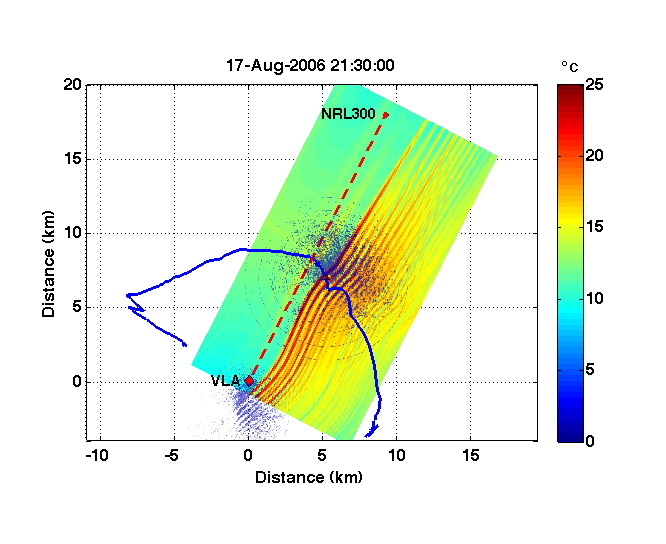
\includegraphics[width=\textwidth]{sw06_Tempr_Depth30m_2006Aug17_213000_radar_curve_thesis1.png}
  \caption{Interpolated internal wave field at 21:30GMT, Aug. 17, water depth = 20m. (Refer to section 3.4 for detailed interpolation method)}\label{fig:r2130_i}
\end{figure}

\begin{figure}[h]
  \centering
  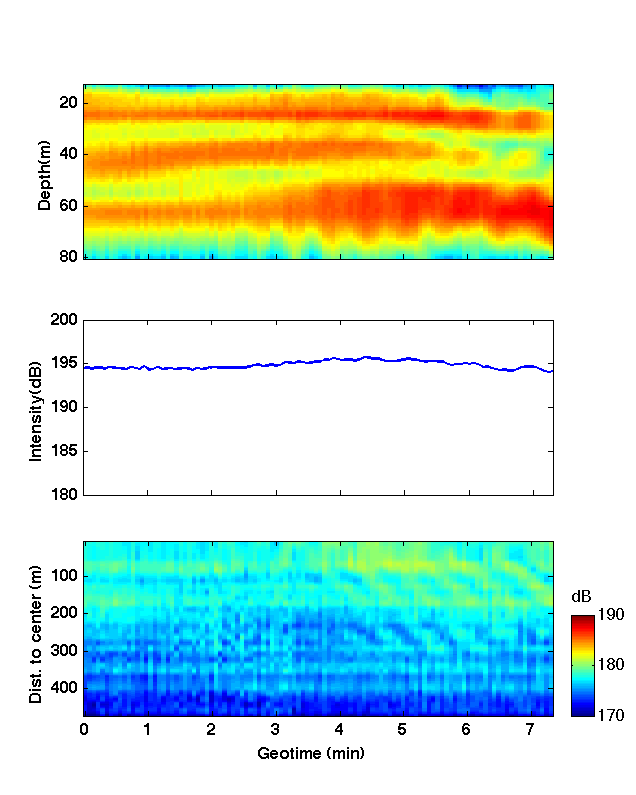
\includegraphics[width=\textwidth]{nrl300_060817T2130_vla_hla_intens_geotime2.png}
  \caption{Received signal on Shark VLA (top), HLA (bottom) and signal intensity (middle) from Aug.17 21:30GMT to 21:37GMT }\label{fig:a2130}
\end{figure}

\begin{figure}[h]
  \centering
  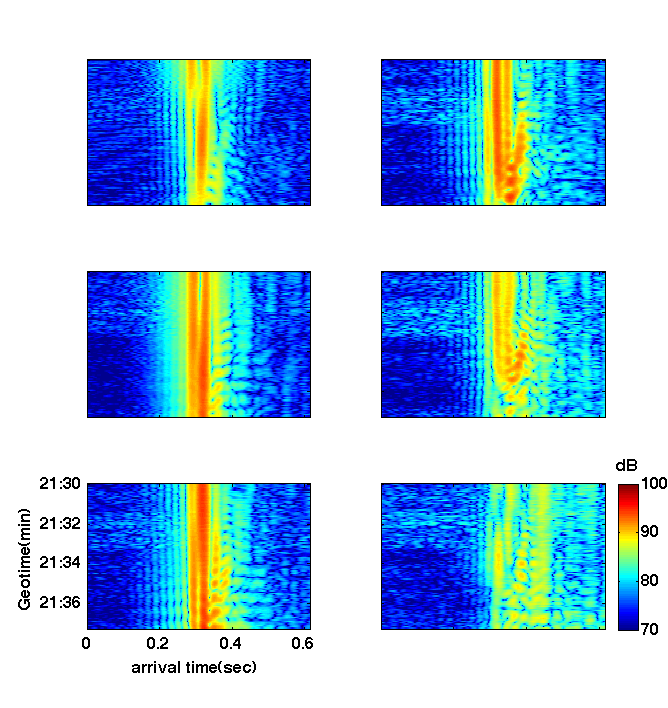
\includegraphics[width=\textwidth]{sw06_broadband_mf_nrl300_F3_6in1_thesis.png}
  \caption{Mode decomposition of received signal on Shark VLA. 
    Left column: mode 1-3, right column: mode 4-6 }\label{fig:m2130}
\end{figure}


%%--F4
\begin{figure}[h]
  \centering
  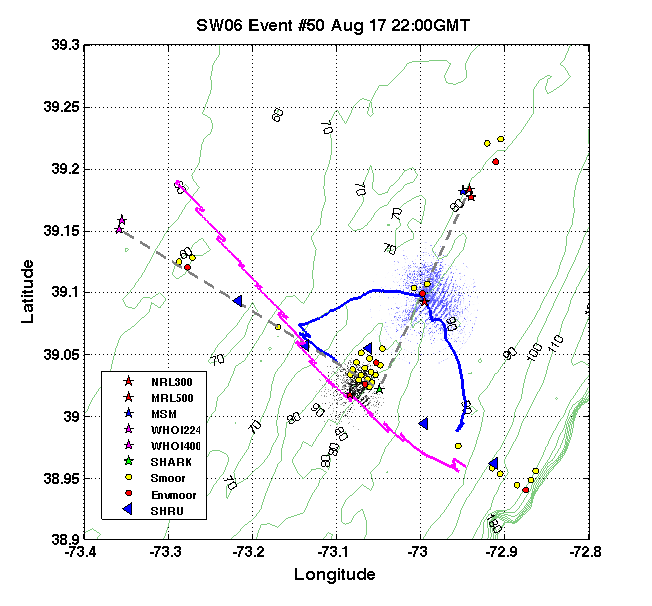
\includegraphics[width=\textwidth]{Aug17_2200_t.png}
  \caption{Surface expression of internal wave package at 21:30GMT, Aug. 17, recorded by R/V Sharp and R/V Oceanus. Blue and red lines indicate their movements, respectively. (Blue: R/V Sharp's, red: R/V Oceanus'}\label{fig:r2130_r}
\end{figure}

\begin{figure}[h]
  \centering
  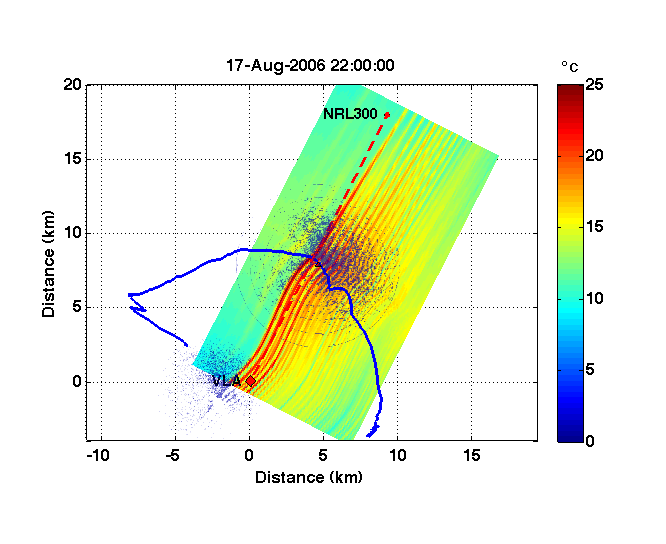
\includegraphics[width=\textwidth]{sw06_Tempr_Depth30m_2006Aug17_220000_radar_curve_thesis1.png}
  \caption{Interpolated internal wave field at 21:30GMT, Aug. 17, water depth = 20m. (Refer to section 3.4 for detailed interpolation method)}\label{fig:r2130_i}
\end{figure}

\begin{figure}[h]
  \centering
  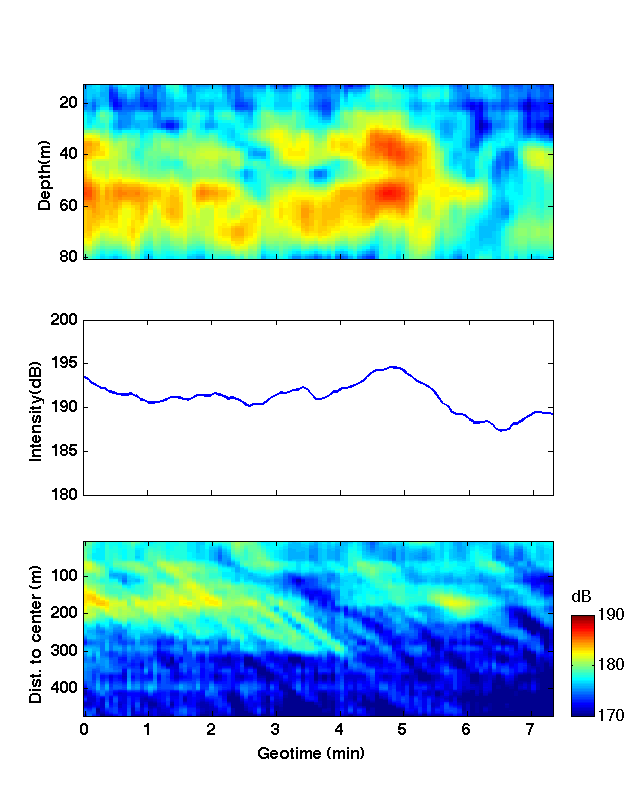
\includegraphics[width=\textwidth]{nrl300_060817T2200_vla_hla_intens_geotime2.png}
  \caption{Received signal on Shark VLA (top), HLA (bottom) and signal intensity (middle) from Aug.17 21:30GMT to 21:37GMT }\label{fig:a2130}
\end{figure}

\begin{figure}[center]
  \centering
  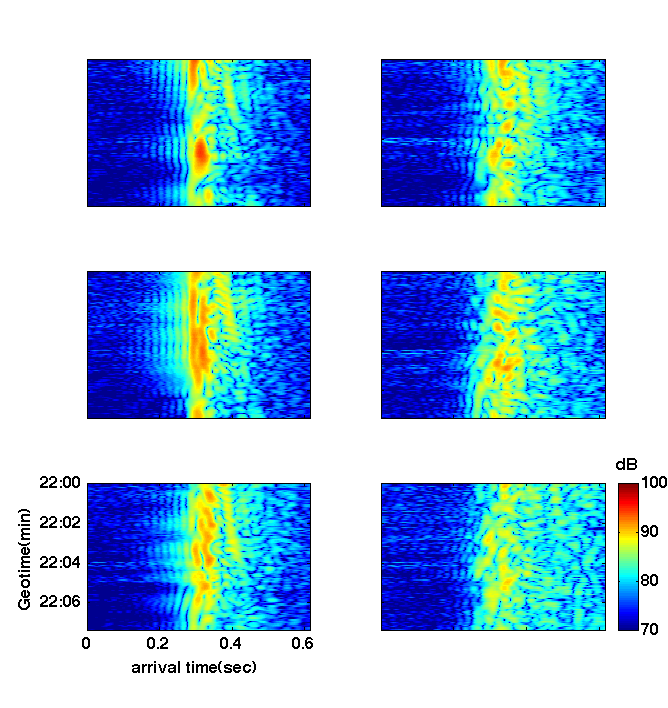
\includegraphics[width=\textwidth]{sw06_broadband_mf_nrl300_F4_6in1_thesis.png}
  \caption{Mode decomposition of received signal on Shark VLA. 
    Left column: mode 1-3, right column: mode 4-6 }\label{fig:m2130}
\end{figure}
\clearpage


%%--F5
\begin{figure}[center]
  \centering
  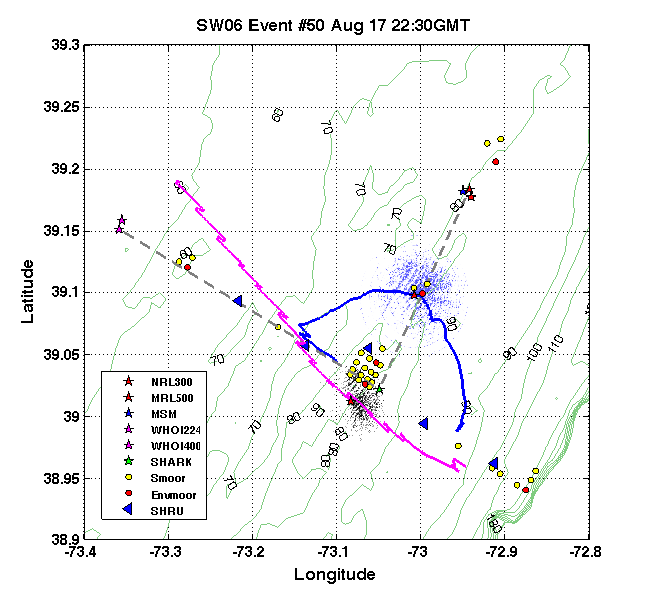
\includegraphics[width=\textwidth]{Aug17_2230_t.png}
  \caption{Surface expression of internal wave package at 21:30GMT, Aug. 17, recorded by R/V Sharp and R/V Oceanus. Blue and red lines indicate their movements, respectively. (Blue: R/V Sharp's, red: R/V Oceanus'}\label{fig:r2130_r}
\end{figure}

\begin{figure}[center]
 \centering
 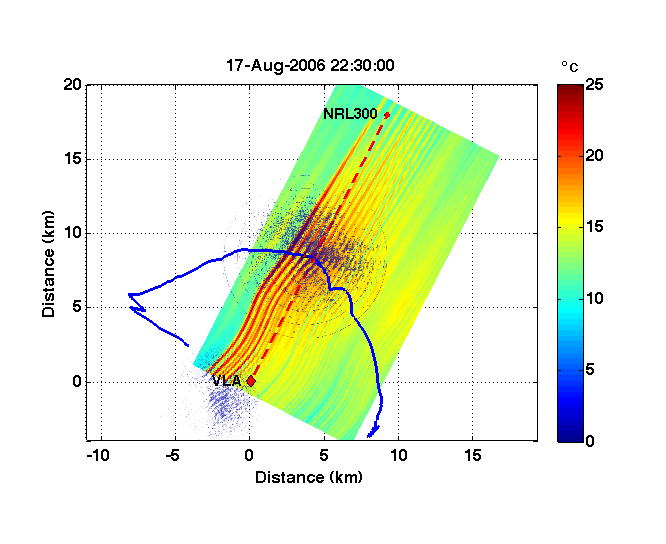
\includegraphics[width=\textwidth]{sw06_Tempr_Depth30m_2006Aug17_223000_radar_curve_thesis1.png}
 \caption{Interpolated internal wave field at 21:30GMT, Aug. 17, water depth = 20m. (Refer to section 3.4 for detailed interpolation method)}\label{fig:r2130_i}
\end{figure}

\begin{figure}[center]
  \centering
  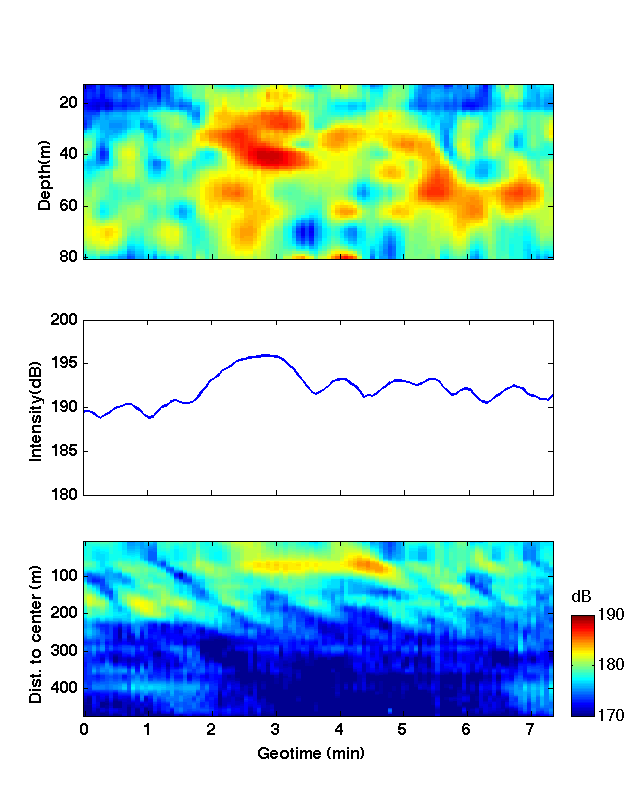
\includegraphics[width=\textwidth]{nrl300_060817T2230_vla_hla_intens_geotime2.png}
  \caption{Received signal on Shark VLA (top), HLA (bottom) and signal intensity (middle) from Aug.17 21:30GMT to 21:37GMT }\label{fig:a2130}
\end{figure}

%\begin{figure}[h]
  %\centering
  %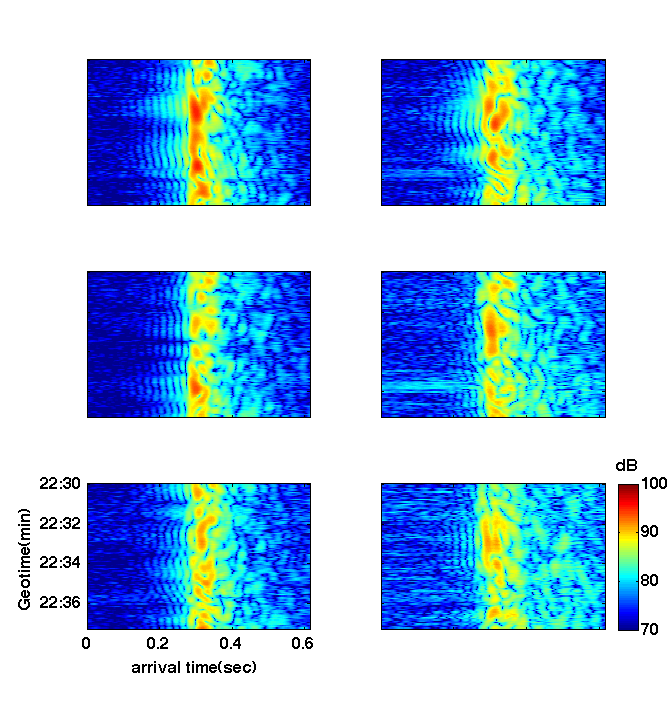
\includegraphics[width=\textwidth]{sw06_broadband_mf_nrl300_F5_6in1_thesis.png}
  %\caption{Mode decomposition of received signal on Shark VLA. 
%    Left column: mode 1-3, right column: mode 4-6 }\label{fig:m2130}
%\end{figure}

